\subsubsection{相互作用ツリークラス}

\subsubsubsection{全体的な流れ}

粒子群クラスから粒子情報をもらい、それを内部のEPI,EPJクラスの配列に情報
を格納する。さらに、EPJ(or I,相互作用によって異なる)から
TP(TreeParticle)クラスを作る。TPクラスは粒子の位置座標のモートンキーと
EPJ(or I)のアドレスを持つ。アドレスは配列のインデックスでS32型で持つこ
とにする。これにより、粒子が同じ順番で並んでいれば、EPIでもEPJでも指す
ことが出来る。またポインタで持つ場合に比べてクラスが軽くなり、配列の再
確保なども容易になる(実装するかは未定)。ここまでで、粒子群クラスの情
報のコピーを持つので、力を計算するまでの間に粒子群クラスから情報をもら
う必要はない。次にTPを使ってローカルツリーを作る。ツリー構造は
TC(TreeCell)クラスの配列によって実現され、これは内部に子セルへの先頭ア
ドレス、自セル内にある先頭のTP(EPI,EPJ)へのアドレスを持つ。さらにTCクラ
スはセルのモーメントやセルの外側境界の情報などを持つMOMENTクラス(長距離
力の場合のみユーザーが定義する事も出来る)を持つ。長距離力の場合はSPJは
MOMENTクラスから情報をもらう事になる。具体的なツリー構築法は決めていな
い(挿入か、それ以外か)が、ツリー構築時点で粒子はツリーを辿った順に並べ
る。これにより、力やモーメント計算などで起こる間接参照を少なく出来る。

ローカルツリー構築、モーメント計算後、相互作用に応じた通信を行い、
EPJ(長距離力の場合はSPJクラスも)を送る。長距離力の場合、送られて来た
EPJ、SPJクラスからTPクラスを作る。ローカルツリーの場合と同様にTPクラス
からグローバルツリーを構築する。モーメント計算においてはTCの指す粒子の
アドレスがEPJかSPJかを区別する必要がある。これはTCの粒子のアドレスの
MSBで区別しようと考えているがまだ未定。

以下はTPとTCの例。

\begin{lstlisting}[caption=TreeParticle]
namespace ParticleSimulator{
    class TreeParticle{
    public:
        U64 key_; //モートンキー
        S32 adr_ptcl_; //対応する粒子のアドレス。
    };
}
\end{lstlisting}

\begin{lstlisting}[caption=TreeCell]
namespace ParticleSimulator{
    template<class Tmom>
    class TreeCell{
    public:
        S32 n_ptcl_; //持っている粒子数
        S32 adr_tc_; //子セルの先頭アドレス
        S32 adr_ptcl_; //粒子の先頭アドレス
        Tmom mom_; //モーメント情報
    };
}
\end{lstlisting}

%%%%%
%モーメント計算時にEPI,EPJどちらの情報を使うか?
%ロングカットオフなしEPJ
%ロングカットオフありEPJ
%Longではツリーは常にJ粒子。
%散乱、固定はEPJ
%集積モードはEPI?
%対称モードはEPI,EPJ?
%力に応じてr_searchの入れる場所を変える。
%%%%%
%モーメント計算用のpropertyクラスがあると便利?
%FP->property
%通信時にもpropertyクラスが必要になる。


\if0
\subsubsubsection{データ構造}

相互作用ツリークラスは、テンプレートクラスであり、以下の様な構造をして
いる。

\begin{lstlisting}[caption=相互作用ツリークラス]
    template<
        int TSM, // search mode
        class Tforce, // USER def
        class Tepi, // USER def
        class Tepj, // USER def
        class Tmom, // PS or USER def
        class Tprop, // PS or USER def
        class Tspj = SuperParticleBase // PS or USER def
        >
    class TreeForForce{
        Tforce * force_i_, * force_buf_;
        Tepi * ep_i_, * ep_i_buf_;
        Tepj * ep_j_, * ep_j_buf_, * ep_j_buf_buf_, * ep_j_loc_, * ep_j_glb_;
        TreeParticle<Tprop> * tp_loc_, * tp_glb_, * tp_buf_;
        TreeCell<TSM, Tmom> * tc_loc_, * tc_glb_, * tc_buf_;
        Tspj * sp_j_;
        S32 n_tot_, n_leaf_max_, n_group_max_;
    };
\end{lstlisting}

テンプレート引数は初めからサーチモード、FORCEクラス、EPIクラス、EPJクラ
ス、MOMENTクラス、PROPERTYクラス、SPJクラスとなっている。

FORCE、EPI、EPJクラスについては仕様書参照。MOMENTクラスはTCクラスがもつ
もので



\subsubsubsubsection{TPクラス}

ツリーの構築、モーメントの計算等に用いる。これらのクラスは{\tt
FullParticle}にアクセスする必要があり、ユーザ定義メソッド({\tt
FullParticle::getPos()}等)を用いてアクセスする。

\begin{lstlisting}[caption=TreeParticle]
namespace ParticleSimulator{
    template<class Tprop>
    class TreeParticle{
    public:
        U64 key_;
        S32 next_adr_tp_;
        Tprop prop_;
        template<class Tfp>
        void setFromFP(const Tfp & fp){
            key_ = MortonKey<DIMENSION>::getKey( fp.getPos() );
            prop_.setFromFP(fp);
        }
    };
}
\end{lstlisting}

{\tt key\_}はモートンキー。{\tt next\_adr\_tp\_}はツリー構築時にリンク
トリストを使う為、隣の粒子の相対アドレス。ツリーの作り方によってはいら
ない可能性がある。これはツリー作成の章で後述。{\tt prop\_}はツリーセル
のモーメント等を作る為に使われる。サーチモードによって適したクラスを使
う。

以下は

\begin{lstlisting}[caption=カットオフなし単極子重力]
namespace ParticleSimulator{
    class PropertyLong{
    public:
        F32 charge_;
        F32vec pos_;
    };
}
\end{lstlisting}



\subsubsubsubsection{TCクラス}

{\tt TP}から粒子情報をもらいセルのモーメントの計算を行い値を格納するク
ラス。

\begin{lstlisting}[caption=TreeCell]
namespace ParticleSimulator{

    template<int TSM, class Tmom>
    class TreeCell{
    public:
        S32 n_ptcl_;
        S32 adr_tc_;
        S32 adr_tp_;
        S32 lev_ni_;
        F32ort vertex_in_;
        Tmom mom_;
    };

}
\end{lstlisting}

テンプレート引数{\tt TSM}はサーチモード。{\tt Tmom}はモーメントクラスで
ツリーセルのモーメント等を保持する。{\tt n\_ptcl\_}はそのセルが持つ粒子
数。{\tt adr\_tc\_}は自分の子セルの最初の相対アドレス。子セルは8個が連
続に並ぶようにするので初めのインデックスだけあれば十分である。{\tt
adr\_tp\_}は自分のもつ粒子の最初のインデックス。

MOMENT、PROPERTY、SPJクラスに関しては以下のものは用意しておき、ユーザー
は自分で定義しなくても以下のものが自由に選択できるようにしておく。

\begin{lstlisting}[caption=プロパティクラス]
    class PropertyLong{
    public:
        F32 charge_;
        F32vec pos_;
        PropertyLong();
        void clear();
        template<class Tfp>
        void copyFromFP(const Tfp & fp);
        F32 getCharge() const { return charge_; }
        F32vec getPos() const { return pos_; }
    };

    class PropertyLongSearch{
    public:
        F32 r_search_;
        F32 charge_;
        F32vec pos_;
        PropertyLongSearch();
        void clear();
        template<class Tfp>
        void copyFromFP(const Tfp & fp);
        F32 getRSearch() const { return r_search_; }
        F32 getCharge() const { return charge_; }
        F32vec getPos() const { return pos_; }
    };

    class PropertySearch{
    public:
        F32 r_search_;
        F32vec pos_;
        PropertySearch();
        void clear();
        template<class Tfp>
        void copyFromFP(const Tfp & fp);
        F32 getRSearch() const { return r_search_; }
        F32vec getPos() const { return pos_; }
    };
\end{lstlisting}

\begin{lstlisting}[caption=モーメントクラス]
    class MomentLMB{
    public:
        F32vec pos_;
        F32 charge_;
        void init();
        F32vec getPos();
        template<class Tprop>
        void accumulateAtLeaf(const Tprop & prop);
        void set();
        void accumulate(const MomentLMB & mom);
        template<class Tprop>
        void accumulateAtLeaf2(const Tprop & prop);
        void accumulate2(const MomentLMB & mom);
    };

    class MomentLQB{
    public:
        F32vec pos_;
        F32 charge_;
        F32mat quad_;
        void init();
        F32vec getPos() const { return pos_; }
        template<class Tprop>
        void accumulateAtLeaf(const Tprop & prop);
        template<class Tprop>
        void accumulateAtLeaf2(const Tprop & prop);
        void set();
        void accumulate(const MomentLQB & mom);
        void accumulate2(const MomentLQB & mom);
    };

\end{lstlisting}


\begin{lstlisting}[caption=SPJクラス]
    class SuperParticleBase{
    public:
        void clear(){}
    };

    class SuperParticleSymEps{
    public:
        F64 charge_;
        F64vec pos_;
        F64 eps_;
        void clear();
    };

    class SuperParticleMonoBaryCenter{
    public:
        F64 charge_;
        F64vec pos_;
        template<class Tmom>
        void copyFromMoment(const Tmom & mom);
        void clear();
        F64    getCharge() const { return charge_; }
        F64vec getPos() const { return pos_; }

    };

    class SuperParticleQuadBaryCenter{
    public:
        F64 charge_;
        F64vec pos_;
        F64mat quad_;
        template<class Tmom>
        void copyFromMoment(const Tmom & mom);
        void clear();
        F64    getCharge() const { return charge_; }
        F64vec getPos() const { return pos_; }
        F64mat getQuad() const { return quad_; }
    };

    class SuperParticleDiGeoCenter{
    public:
        F64 charge_;
        F64vec pos_;
        F64vec di_;
    };

    class SuperParticleQuadGeoCenter{
    public:
        F64 charge_;
        F64vec pos_;
        F64vec di_;
        F64mat quad_;
    };

\end{lstlisting}

テンプレート引数が多いので、ユーザーが全て指定しなくても良いように、よ
く使う組み合わせはtypedefしておく。

\begin{lstlisting}[caption=相互作用ツリークラス]

    template<
        class Tforce, // user def
        class Tepi, // user def
        class Tepj // user def
        >
    class TreeType{
    public:
        typedef TreeForForce <
            SEARCH_MODE_LONG,
            Tforce, Tepi, Tepj,
            TreeCell<SEARCH_MODE_LONG, MomentLMB>,
            TreeParticle<PropertyLong>,
            SuperParticleMonoBaryCenter > TreeForMonoBaryCenter;

        typedef TreeForForce <
            SEARCH_MODE_LONG,
            Tforce, Tepi, Tepj,
            TreeCell<SEARCH_MODE_LONG, MomentLQB>,
            TreeParticle<PropertyLong>,
            SuperParticleQuadBaryCenter > TreeForQuadBaryCenter;

        typedef TreeForForce <
            SEARCH_MODE_GATHER,
            Tforce, Tepi, Tepj,
            TreeCell<SEARCH_MODE_GATHER, MomentSearch>,
            TreeParticle<PropertySearch>,
            SuperParticleBase > TreeForGatherSearch;

        typedef TreeForForce <
            SEARCH_MODE_SCATTER,
            Tforce, Tepi, Tepj,
            TreeCell<SEARCH_MODE_SCATTER, MomentSearch>,
            TreeParticle<PropertySearch>,
            SuperParticleBase > TreeForScatterSearch;

        typedef TreeForForce <
            SEARCH_MODE_SYMMETRY,
            Tforce, Tepi, Tepj,
            TreeCell<SEARCH_MODE_SYMMETRY, MomentSearch>,
            TreeParticle<PropertySearch>,
            SuperParticleBase > TreeForSymmetrySearch;
    };

\end{lstlisting}
\fi


\subsubsubsection{初期化}

以下の関数により初期化を行う。

\begin{screen}
\begin{verbatim}
void initialize(DomainInfo * dinfo,
                const F32 theta = 0.5,
                const S32 nleafmax = 8,
                const S32 ngroupmax = 64);
\end{verbatim}
\end{screen}

メンバ{\tt theta\_}、{\tt n\_leaf\_max\_}、{\tt n\_group\_max\_}を設定。
さらに、FORCE, EPI, EPJ, TP, TC, SPJの配列を確保する。\redtext{配列サイ
ズの決め方はまだ決めていない。}

\subsubsubsection{相互作用計算に必要な粒子データの読込}

粒子群クラスから相互作用ツリークラスへの粒子データの読み込みは以下の関
数によって行う。

\begin{screen}
\begin{verbatim}
void setParticleFromFullParticle(const Tpsys & psys, const bool clear);
\end{verbatim}
\end{screen}

引数の意味は仕様書参照。粒子群クラスのメンバ{\tt ptcl\_}から、{\tt
epi\_org\_}、{\tt epj\_org\_}、に必要なデータを抜き出す。この時、{\tt
epi\_org\_}、{\tt epj\_org\_}については、ユーザーが定義したメソッド
{\tt EPI::copyFromFP(...)}, {\tt EPJ::copyFromFP(...)}によって行われ、
{\tt tp\_loc\_}については、{\tt TP::setFromEP(...)}によって行われる。

%引数の意味は仕様書参照。粒子群クラスのメンバ{\tt ptcl\_}から、{\tt
%tp\_loc\_}、{\tt epi\_buf\_}、{\tt epj\_buf\_}、に必要なデータを抜き出
%す。この時、{\tt epi\_buf\_}、{\tt epj\_buf\_}については、ユーザーが定
%義したメソッド{\tt EPI::copyFromFP(...)}, {\tt EPJ::copyFromFP(...)}に
%よって行われ、{\tt tp\_loc\_}については、{\tt TP::setFromEP(...)}によっ
%て行われる。

\subsubsubsection{ツリーのルートセルの決定}

以下の二つはツリーのルートセルを決定する為の関数である。この関数を呼ぶ
ことで、ツリーのルートセルの情報が決まる(メンバ変数{\tt
pos\_root\_cell\_}, {\tt center\_}, {\tt length\_}に値が入る)。{\tt
FDPS}では、ローカルツリー、グローバルツリーで同じルートセルを使う。最初
の関数は領域クラスから、境界条件の情報をもらい、適切なルートセルを決定
する。開放境界の場合は、全ての粒子を内包する最少の立方体をルートセルに
する。周期境界条件の場合は、全ての粒子を内包する最少の立方体に最大の探
査半径のマージを取った立方体を使う。

\begin{screen}
\begin{verbatim}
void setRootCell(const DomainInfo & dinfo);
\end{verbatim}
\end{screen}


下の関数を使うと、直接ツリーのルートセルの中心(cen)と一辺の長さ(len)を
指定する事が出来る。ここで指定された範囲外に粒子がある場合の動作は未定
義である。

\begin{screen}
\begin{verbatim}
void setRootCell(const F32 len, const F32vec & cen=F32vec(0.0));
\end{verbatim}
\end{screen}

\subsubsubsection{ローカルツリーの作成}

以下、2種類の方法を考える。最初は後者の方法を実装する。

{\bf 粒子挿入によるツリー作成}

まず、{\tt tp\_org\_}の粒子挿入によりツリーを作る。一つのセルに{\tt
n\_leaf\_max\_}個以上の粒子が入ってきたら8個の子セルを{\tt tc\_loc\_}か
ら連続に取り、その最初の小セルの配列先頭からの相対アドレスを{\tt
adr\_tc\_}に格納。次に、ツリーを順に辿りその順番に粒子を並び替え{\
tp\_i\_}に格納する。

スレッド並列にする場合はまず{\tt n\_leaf\_max\_}より十分大きな粒子数(粒
子数/スレッド数位?)のセルをリーフ(ここではブランチと呼ぶ)とするツリー
を作り、各ブランチセルに対して各スレッドでツリーを独立に作れば良い。粒
子の並び替えのスレッド並列では以下の様にする。各ブランチ粒子数のprefix
sum(オフセット)を計算する。各ブランチを各スレッドで辿り粒子を並び替え、
先程計算したオフセットを使って{\tt tp\_i\_}の適切な場所に格納すればよい。
{\tt ep\_i\_}も同じ順番に並べ替える。

{\bf モートンソートによるツリー作成}

まず、{\tt epi\_org\_}の位置座標からモートンキーを計算し、{\tt
tp\_loc\_}の{\tt key}に値を代入する。 {\tt tp\_loc\_}のモートンキーを使っ
てソートを行い同じ順番にEPも並べ替える。この際並べ替えたEPは{\tt
epi\_sorted\_},{\tt epj\_sorted\_}に格納する。これら行う関数が以下であ
る。

\begin{screen}
\begin{verbatim}
void mortonSortLocalTreeOnly();
\end{verbatim}
\end{screen}

ソートには粒子数の少ないところ($\sim 8000$)ではsample sort,粒子数の多い
ところではradix sortを使うつもりであるが現在はradix sortのみ実装。また、
radix sortのprefix sumはまだスレッド並列化していない。ローカルツリーの
モートンソートは以下の関数によって実行される。

図\ref{fig:sorting_time}は「京」1ノードでのstd::sort(1スレッド使用),
sample sort(8スレッド使用), radix sort(8スレッド使用)の比較。ソートした
構造体は64bitのkeyと32bit整数からなる。

sample sortはまず、各スレッドで各部分をソートする。その後ランダムに粒子
を選び、ランダムサンプルされたものをシングルスレッドで再びソート。サン
プルの値を使って、各スレッドで同じ粒子数位持つように、値の範囲を決め粒
子を並べ替える。この時prefix sumを使って粒子の位置のオフセットを決める。
並べ替えたら、各スレッドでソートをすればグローバルにソートされたことに
なる。ここのソートはマージソートを使う。

\begin{figure}[h]
  \begin{center}
    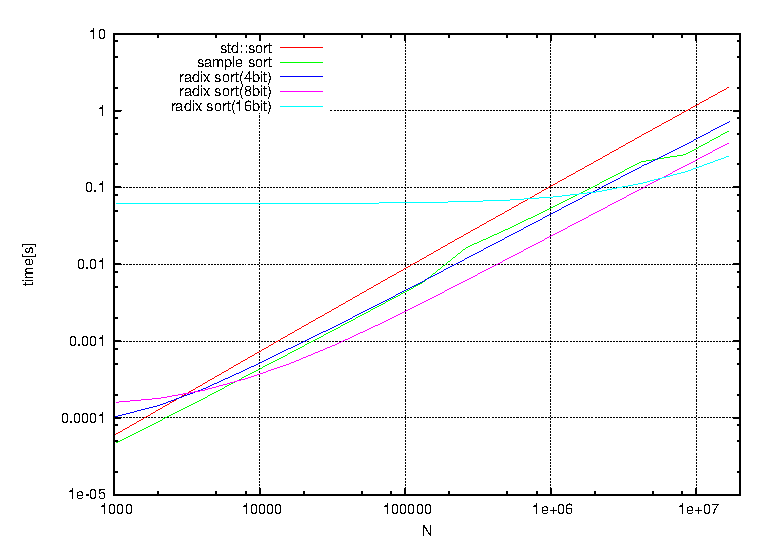
\includegraphics[width=15cm]{fig/sorting_time.eps}
  \end{center}
  \caption{ソート時間の比較}
  \label{fig:sorting_time}
\end{figure}

\newpage

次にツリー構造をトップからレベル毎に作っていく。ツリーのセルを作るのに
はバイナリーサーチを使う。粒子数が少なくなってきたらリニアサーチを使っ
た方が良いかもしれないが実装していない。子セルをアロケートする場所を決
めるのにprefix sumを使っているが、スレッド並列化はしていない。以下の関
数により、ツリー構造が作られる。この関数はモートンソート前に呼んではな
らない。

\begin{screen}
\begin{verbatim}
void linkCellLocalTreeOnly();
\end{verbatim}
\end{screen}

モーメントの計算は下のレベルから順に行う。ツリーセルはレベル毎に連続で
メモリー上に並んでいるので、各レベルでスレッド並列で行う。モーメントの
計算は次の関数で行う。

\begin{screen}
\begin{verbatim}
void calcMomentLocalTreeOnly();
\end{verbatim}
\end{screen}


図\ref{fig:makeLT}は京で8スレッド使った時にローカルツリー作りにかかる時
間。

\begin{figure}[h]
  \begin{center}
    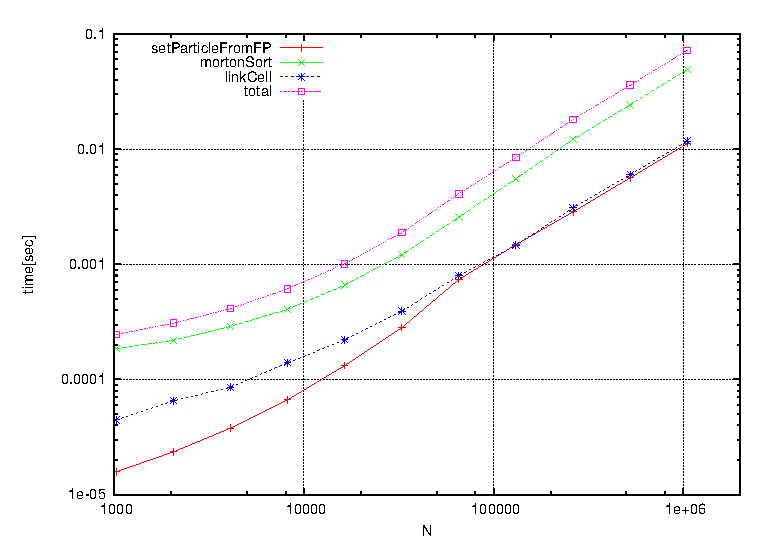
\includegraphics[width=15cm]{fig/timeingLT.eps}
  \end{center}
  \caption{ローカルツリー構築}
  \label{fig:makeLT}
\end{figure}

\newpage

図\ref{fig:makeLT}はXeon(2.93GHz, Nehalem)で6スレッド使った時にローカル
ツリー作りにかかる時間。モーメント計算は重心の計算のみ。

\begin{figure}[h]
  \begin{center}
    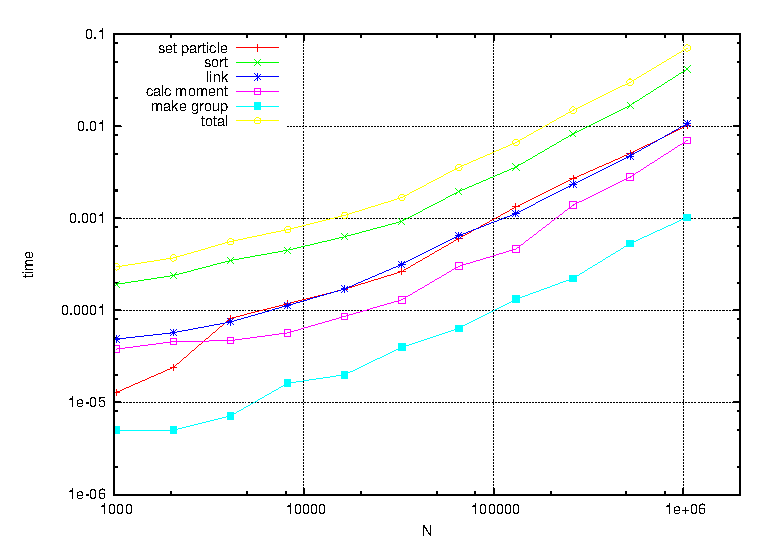
\includegraphics[width=15cm]{fig/timeingLT_xeon.eps}
  \end{center}
  \caption{ローカルツリー構築}
  \label{fig:makeLT}
\end{figure}

\newpage

{\bf radix sort クラス}

radix sort クラスは以下の様になっている。

\begin{lstlisting}[caption=RadixSort]
namespace ParticleSimulator{
    template<class T, int NBIT=8>
    class RadixSort{
    private:
        int n_thread_;
        int n_bucket_;
        T mask_;
        int ** bucket_size_;
        int ** prefix_sum_;
    public:
        RadixSort();
        template<class Tobj>
        void lsdSort(Tobj * & val,
                     Tobj * & val_buf,
                     const int first,
                     const int last);
    };
}
\end{lstlisting}

注意として、このクラスはunsigned型の整数のみに対応している。また、メソッ
ド{\tt lsdSort}でOpenMPを使っている。

クラステンプレートパラメータは最初がソートする対象の型(U64)、
{\tt NBIT}はradixのビット数でデフォルトは8bit。コンストラクタにより、メ
ンバの領域や値が代入される。

%%%%%%%%%%%%%%%
\begin{screen}
\begin{verbatim}
template<class Tobj>
void lsdSort(Tobj * & val,
             Tobj * & val_buf,
             const int first,
             const int last);

\end{verbatim}
\end{screen}

\begin{itemize}

\item{{\bf 引数}}

{\tt val}: 入力、出力。

{\tt val\_buf}: 入力。

{\tt first}: 入力。

{\tt last}: 入力。

\item{{\bf 返り値}}

なし。

\item{{\bf 機能}}

{\tt val}のメソッド{\tt getKey()}により返される値の順に{\tt val}をソー
トする。{\tt val\_buf}は{\tt val}と同じ型、サイズの配列でソートする時の
バッファー領域として使う。{\tt first}はソートする配列の領域の最初のイン
デックス、{\tt last}はソートする配列の領域の最後のインデックス。内部で
はOpenMPを用いて並列化されている。

\end{itemize}

使い方はまずオブジェクトを作り、メソッド{\tt lsdSort()}を呼び出す。
\begin{lstlisting}[caption=RadixSortの例]

    PS::TreeParticle * data = new TreeParticle[n_size];
    PS::TreeParticle * data_buf = new TreeParticle[n_size];
    for(int j=0; j<n_size; j++){
        data[j].setKey(PS::U64(abs(rand()))<<32 | PS::U64(abs(rand())));
    }
    PS::RadixSort<PS::U64, 8> RS;
    RS.lsdSort(data, data_buf, 0, n_size-1);

\end{lstlisting}

\subsubsubsection{相互作用計算に必要な粒子の交換}

前提として、全プロセスのドメインの座標を全プロセスが持っている(領域分割
時に全座標を放送する)。

\subsubsubsubsection{開放境界、長距離力カットオフなし}

他ドメインに対して自プロセスのツリーをたどり、他ドメインが力を計算する
のに十分なEPJ、SPJをそれぞれ、{\tt ep\_j\_send\_}、{\tt sp\_j\_send\_}
に格納する。またその個数を{\tt n\_ep\_j\_send\_[]}、{\tt
n\_sp\_j\_send\_[]}に格納する。配列のインデックスはプロセス番号と対応さ
せること。まず、{\tt n\_ep\_j\_send\_[]}、{\tt n\_sp\_j\_send\_[]}を
Alltoallし、受信した値を{\tt n\_ep\_j\_recv\_[]}、{\tt
n\_sp\_j\_recv\_[]}に格納する。次にAlltoallvを使い{\tt ep\_j\_send\_}、
{\tt sp\_j\_send\_}を送り、受信した値を{\tt ep\_j\_recv\_}、{\tt
sp\_j\_recv\_}に格納する。

\subsubsubsubsection{開放境界、長距離力カットオフあり}

自ドメインと他ドメインの距離を測り、カットオフ半径より短い場合はローカ
ルツリーをたどる。辿り方はほとんど”長距離力カットオフなし”の場合と同
じだか、ツリーセルと他ドメインの距離がカットオフ長より長い場合はそのセ
ルを辿る必要は無い。通信は粒子数を送る所は”長距離力カットオフなし”の
場合と同じだが、粒子は全てのノードに送るわけではないのでAlltoallvを使わ
ずにIsend, Irecvで送る。

\subsubsubsubsection{開放境界、短距離力散乱モード}

%他プロセスのツリールートセルの内側境界(ドメインでも良い)に対して自プロ
%セスのツリーを辿る。この時ツリーの外側境界を使って、

他プロセスのドメインに対して自プロセスのツリーを辿る。この時ツリーの外
側境界を使って、他プロセスのドメインとの距離を測る。通信パターンは"開放
境界、長距離力カットオフあり"の場合と同じ。


\subsubsubsubsection{開放境界、短距離力収集モード}

最初に、ツリールートセルの外側境界の座標をAllgatherする。他プロセスのツ
リールートセルの外側境界に対して自プロセスのツリーを辿る。この時ツリー
の内側境界を使って、他プロセスのドメインとの距離を測る。

上記の方法だと、例えばプロセス内の粒子にカットオフ半径のばらつきがあっ
た場合など、通信量が非常に増えてしまう場合も考えられる。そこで、以下の
様な方法も考えられる。まず、”短距離力散乱モード”と同様の方法で、粒子
を送る(Alltoallで粒子数を送り、Isend,IredvでEPJを送る)。次に送られて来
た粒子のカットオフ半径内に入り、かつ送られて来た粒子の送信元プロセスの
ルートセルのドメインとの距離がそのカットオフ半径より長い粒子(「送信元」
プロセスには送られていない粒子)を{\tt ep\_j\_send\_}に格納する。

%送信する粒子が重複しないようにソート等を行う。粒子を送ったプロセスから
%しか粒子は送られてこないので、粒子数、EPJをIsend,Irecvで通信する。この
%ようにすると送られて来た粒子は散乱モードと収集モードの和集合を含むので
%十分である。




\subsubsubsubsection{開放境界、短距離力対称モード}

最初に、ツリールートセルの外側境界の座標をAllgatherする。他プロセスのツ
リールートセルの外側境界に対して自プロセスのツリーを辿る。この時ツリー
の外側境界を使って、他プロセスの外側境界との距離を測る。

収集モードの場合で述べた2段階通信の方法も考えられる。

%ルートセルの外側境界とが重なっているかを判定する。
%重なっている場合はツリーを辿り、重なりのあるリーフセルの粒子と他プロセ
%スの外側境界との距離がその粒子のカットオフ半径より短い場合はその粒子を
%送る。

%集積モードの場合と同様に、カットオフ半径にばらつきがあると通信量が増え
%てしまう可能性がある。そこで集積モードの場合と同様に2段階で通信する方
%法も考えられる。まず、”短距離力散乱モード”と同様の方法で、粒子を送る。
%次に送られて来た粒子のカットオフ半径内に入り、かつ送られて来た粒子の送
%信元プロセスのルートセルの内側境界(もしくはドメイン)との距離がそのカッ
%トオフ半径より長い粒子(「送信元」プロセスには送られていない粒子)を送信
%する。

\subsubsubsubsection{開放境界、短距離力固定モード}

短距離力散乱モードと同じ実装を行う。

\subsubsubsubsection{直方体周期境界、長距離力カットオフあり}

\subsubsubsubsection{直方体周期境界、短距離力散乱モード}

\subsubsubsubsection{直方体周期境界、短距離力収集モード}

\subsubsubsubsection{直方体周期境界、短距離力対称モード}

\subsubsubsubsection{直方体周期境界、短距離力固定モード}

\subsubsubsection{グローバルツリーの作成}

\subsubsubsubsection{開放境界条件}

{\tt ep\_j\_recv\_},{\tt sp\_j\_recv\_}から{\tt tp\_glb\_}を作る。この
際TPの{\tt adr\_ptcl\_}は{\tt ep\_j\_recv\_},{\tt sp\_j\_recv\_}の配列
のインデックスを入れるが、EPJとSPJを区別するためにSPJのMSBは1にする。ツ
リー構築はローカルツリーと同様。最初はモートーンソートを作ってからのツ
リー構築を実装する。LETが少ない場合は挿入の方が速いかもしれない。

\subsubsubsubsection{直方体周期境界条件}


\subsubsubsection{i粒子グループ構築}

{\tt PS}ではいくつかのi粒子群に対してツリーを辿るので、相互作用の計算の
前にi粒子グループの構築を行う。これは、ローカルツリーの構造を使うだけな
ので、ローカルツリー構築以降、相互作用計算の前ならどこでも行う事が出来
るので、LET交換にオーバーラップさせることも出来る。ただし、この計算コス
トは軽いのであまり意味がないかもしれない。

以下にi粒子群を表すクラスを示す。

\begin{lstlisting}[caption=IPGroup]
namespace ParticleSimulator{
    template<int Tsmode>
    class IPGroup{
    public:
        F32ort vertex_;
        S32 adr_ptcl_;
        S32 n_ptcl_;
        template<class Ttc> void copyFromTC(const Ttc & tc);
    };
\end{lstlisting}

{\tt vertex\_}はi粒子グループを囲む直方体の座標で、力の種類によって表現
するものが異なる。力の種類はテンプレートパラメータとして与えられる。短
距離力散乱モードでは内側境界、短距離力収集モードと短距離力対称モードと
短距離力固定長モードでは外側境界を使う。長距離力では内側境界を使うと計
算量がツリーセルがスパースなところでは計算量が減るが絶対必要というわけ
ではないので、長距離量の場合の実装をどうするかは未定。{\tt
adr\_ptcl\_}は{\tt ep\_i\_}のインデクスで、{\tt n\_ptcl\_}はそのi粒子群
の個数である。{\tt ep\_i\_}は順番に並んでいるのでインデックスと粒子数だ
けあれば計算可能である。

以下の関数により、i粒子グループを作る。

\begin{screen}
\begin{verbatim}
void makeIPGroup();
\end{verbatim}
\end{screen}

\subsubsubsection{相互作用の計算}



\subsubsubsection{相互作用の書込}


\subsubsubsection{近傍粒子探査}

{\tt SEARCH\_MODE}が{\tt LONG_SCATTER}、{\tt LONG_CUTOFF_SCATTER}、
{\tt LONG_SYMMETRY}、{\tt LONG_CUTOFF_SYMMETRY}の場合には以下に述べる
近傍粒子探査用の関数が使える。
\redtext{{\tt LONG_SYMMETRY}、{\tt LONG_CUTOFF_SYMMETRY}は未実装}。
